% -*- mode: latex; -*- mustache tags:  
\documentclass[10pt,twoside,english]{_support/latex/sbabook/sbabook}
\let\wholebook=\relax

\usepackage{import}
\subimport{_support/latex/}{common.tex}

%=================================================================
% Debug packages for page layout and overfull lines
% Remove the showtrims document option before printing
\ifshowtrims
  \usepackage{showframe}
  \usepackage[color=magenta,width=5mm]{_support/latex/overcolored}
\fi


% =================================================================
\title{A PharoThings Tutorial}
\author{Allex Oliveira}
\series{Square Bracket tutorials}

\hypersetup{
  pdftitle = {A PharoThings Tutorial},
  pdfauthor = {Allex Oliveira},
  pdfkeywords = {IoT, Raspberry, PharoThings, Pharo}
}


% =================================================================
\begin{document}

% Title page and colophon on verso
\maketitle
\pagestyle{titlingpage}
\thispagestyle{titlingpage} % \pagestyle does not work on the first one…

\cleartoverso
{\small

  Copyright 2017 by Allex Oliveira.

  The contents of this book are protected under the Creative Commons
  Attribution-ShareAlike 3.0 Unported license.

  You are \textbf{free}:
  \begin{itemize}
  \item to \textbf{Share}: to copy, distribute and transmit the work,
  \item to \textbf{Remix}: to adapt the work,
  \end{itemize}

  Under the following conditions:
  \begin{description}
  \item[Attribution.] You must attribute the work in the manner specified by the
    author or licensor (but not in any way that suggests that they endorse you
    or your use of the work).
  \item[Share Alike.] If you alter, transform, or build upon this work, you may
    distribute the resulting work only under the same, similar or a compatible
    license.
  \end{description}

  For any reuse or distribution, you must make clear to others the
  license terms of this work. The best way to do this is with a link to
  this web page: \\
  \url{http://creativecommons.org/licenses/by-sa/3.0/}

  Any of the above conditions can be waived if you get permission from
  the copyright holder. Nothing in this license impairs or restricts the
  author's moral rights.

  \begin{center}
    
\includegraphics[width=0.2\textwidth]{_support/latex/sbabook/CreativeCommons-BY-SA.pdf}
  \end{center}

  Your fair dealing and other rights are in no way affected by the
  above. This is a human-readable summary of the Legal Code (the full
  license): \\
  \url{http://creativecommons.org/licenses/by-sa/3.0/legalcode}

  \vfill

  % Publication info would go here (publisher, ISBN, cover design…)
  Layout and typography based on the \textcode{sbabook} \LaTeX{} class by Damien
  Pollet.
}


\frontmatter
\pagestyle{plain}

\tableofcontents*
\clearpage\listoffigures

\mainmatter

\chapter{Lesson 4 - LED Flowing Lights}
Now we can play with the LEDs, turn them on, off, and blink. Let's put 8 LEDs on the breadboard and create a code to turn on/off one at a time. Let's use some methods to change the flow direction and control the flow time. As we did in the last lesson, let's write the first code in playground and then create a class with methods to better control the flow of LED lights. 
\section{What do we need?}
We are using the set of the first lesson, but let's use 8 LEDs and 8 resistors and some more jumper wires.
\subsection{Components}
\begin{itemize}
\item 1 Raspberry Pi connected to your network (wired or wireless)
\item 1 Breadboard
\item 8 LEDs
\item 8 Resistors 330ohms
\item Jumper wires
\end{itemize}
\section{Experimental procedure}
We saw in lesson 1 how to connect the LED and resistors on the breadboard. Now let's do the same, but putting more 7 LEDs and resistors on the breadboard. 

\begin{itemize}
\item Connect the Ground PIN from Raspberry in the breadboard blue rail (-). 
\item Then connect the 8 resistors from the blue rail (-) to a column on the breadboard, as shown below;
\item Now push the LED legs into the breadboard, with the long leg (with the kink) on the right;
\item And insert the jumper wires connecting the right column of each LED to GPIO from 0 to 7, as shown in the Picture \ref{Schema8Leds}.
\end{itemize}

The Figure \ref{Physical8Leds} shows how the electric connection is made.


\begin{figure}

\begin{center}
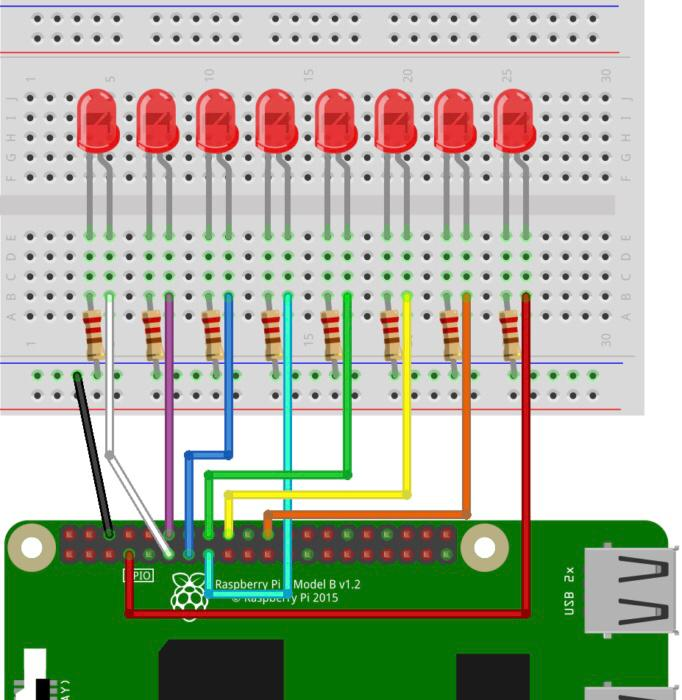
\includegraphics[width=0.6\textwidth]{/Users/allexoliveira/PharoThingsBook/Booklet-APharoThingTutorial/_result/pdf/Chapters/Chap5LEDFlowingLights/figures/pharothings-raspberry-8leds-8resistors-board.jpeg}\caption{Schema connection 8 LEDs.\label{Schema8Leds}}\end{center}
\end{figure}


\begin{figure}

\begin{center}
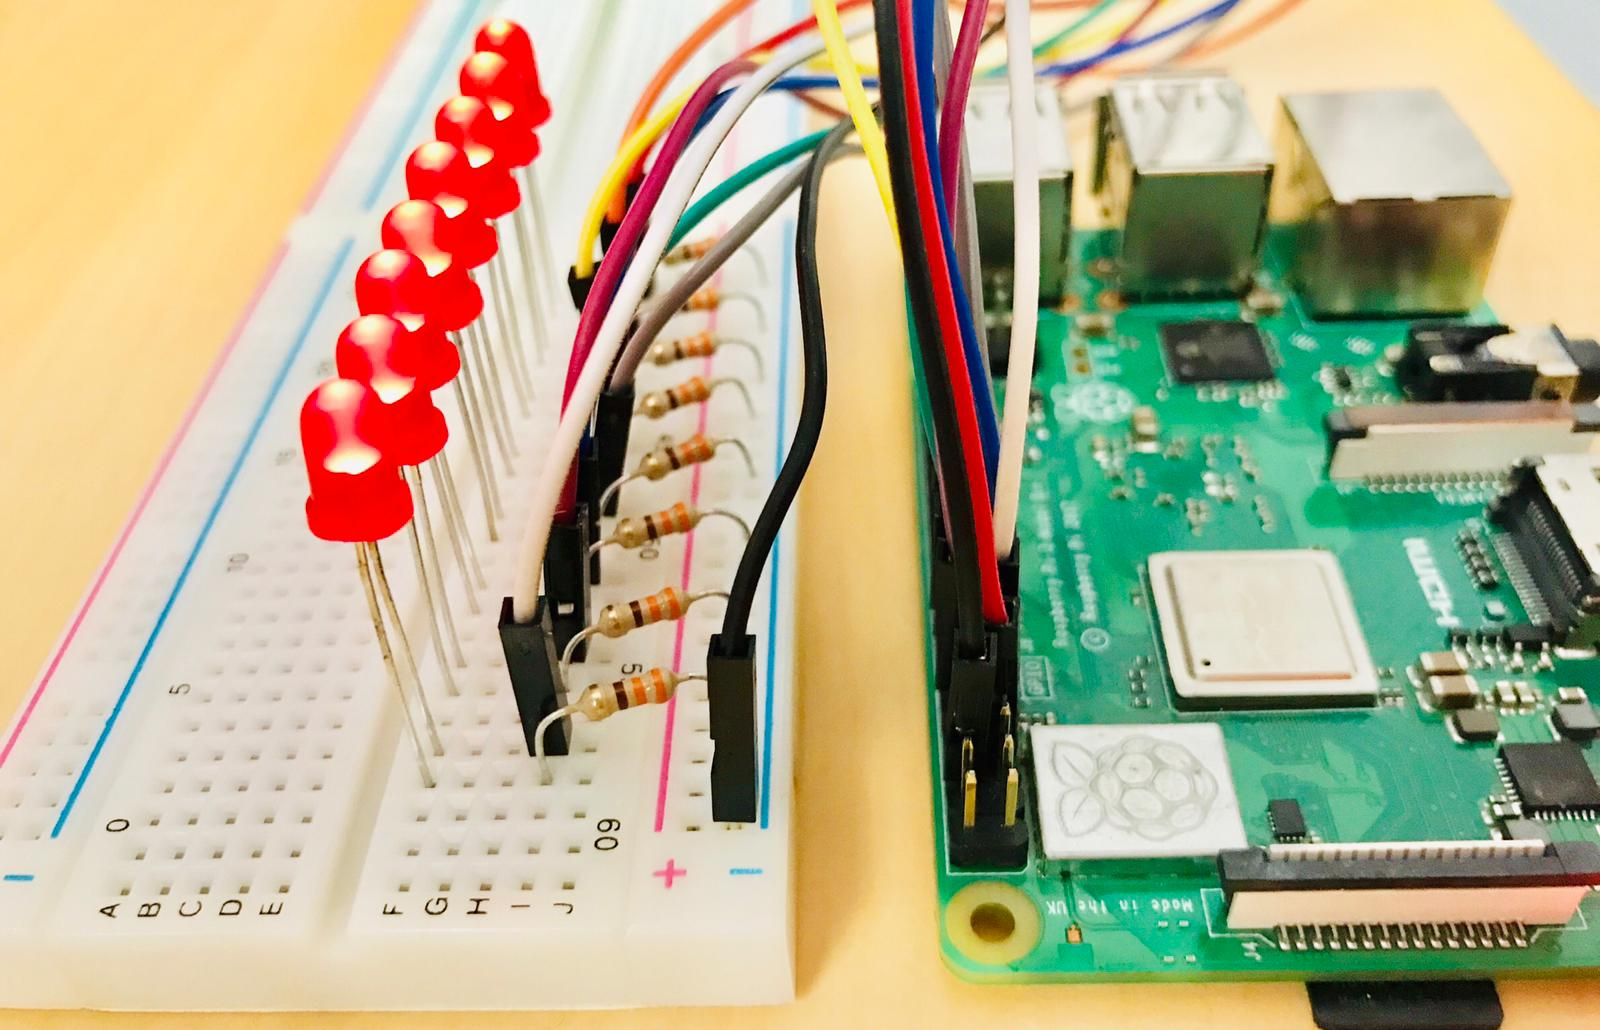
\includegraphics[width=0.6\textwidth]{/Users/allexoliveira/PharoThingsBook/Booklet-APharoThingTutorial/_result/pdf/Chapters/Chap5LEDFlowingLights/figures/pharothings-raspberry-raspberry-leds-breadboard-01.jpeg}\caption{Physical connection 8 LEDs.\label{Physical8Leds}}\end{center}
\end{figure}

\subsection{Connecting remotely}
Through your local Pharo image, let's connect in the Pharo image by running on Raspberry, enable the auto-refresh feature of the inspector, and open the inspector.

Run this code in your local playground:

\begin{displaycode}{plain}
remotePharo := TlpRemoteIDE connectTo: (TCPAddress ip: #[193 51 236 212] port: 40423)
GTInspector enableStepRefresh.
remoteBoard := remotePharo evaluate: [ RpiBoardBRev1 current].
remoteBoard inspect.
\end{displaycode}
\section{Experimental code}
In your inspect window (Inspector on a PotRemoteBoard), let’s create an array and initialize the 8 LEDs, putting each one in a position of the array.  This way we can send messages more easily to all objects. Look at the second line, we set the GPIOs to \textcode{beDigitalOutput} only using the method \textcode{do:} to move through the entire array:

\begin{displaycode}{plain}
gpioArray := { gpio0. gpio1. gpio2. gpio3. gpio4. gpio5. gpio6. gpio7 }.
gpioArray do: [ :item | item beDigitalOutput ].
\end{displaycode}

To change the value of the object (led value), let's call the method \textcode{toggleDigitalValue}, as we saw previously. You can also use the method \textcode{value:} and send 1 or 0, instead \textcode{toggleDigitalValue}, but let's use this last. To do this fast and simple, let's use again the method \textcode{do:} to send the parameters to all objects on the array. In this example, we turn On all the LEDs at the same time:

\begin{displaycode}{plain}
gpioArray do: [ :item | item toggleDigitalValue ].
\end{displaycode}

Let's put a Delay after changing the led value, to wait a bit time before to change the next LED value.  Let's also put this inside a process using the method \textcode{forkNamed}:

\begin{displaycode}{plain}
[
    gpioArray do: [ :item | item toggleDigitalValue. (Delay forSeconds: 0.3) wait ].
] forkNamed: 'FlowingProcess'.
\end{displaycode}

Execute this code and… cool! Now your LEDs are on by flowing an ordering!

Change the value of the method \textcode{forSeconds}: to wait less time between toggling it. This will cause the line LEDs to turn on faster. The Figure \ref{Inspector8LEDs} and \ref{8LEDs} shows the code and the LEDs turn On.


\begin{figure}

\begin{center}
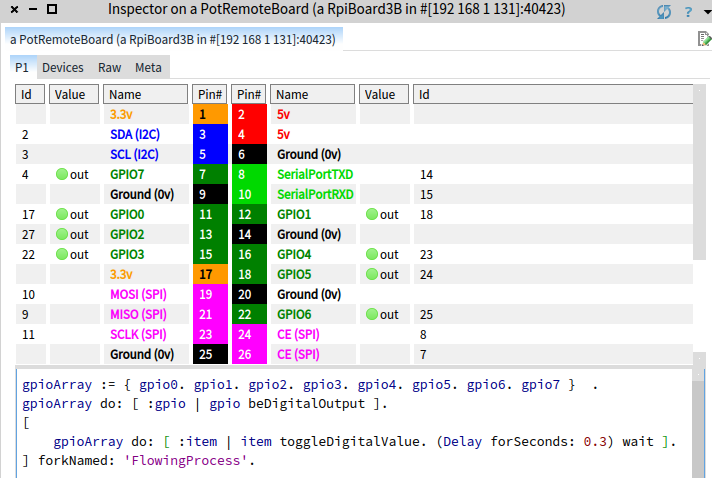
\includegraphics[width=0.85\textwidth]{/Users/allexoliveira/PharoThingsBook/Booklet-APharoThingTutorial/_result/pdf/Chapters/Chap5LEDFlowingLights/figures/pharothings-raspberry-8leds-code-lesson-01.png}\caption{Code on Inspector\label{Inspector8LEDs}}\end{center}
\end{figure}


\begin{figure}

\begin{center}
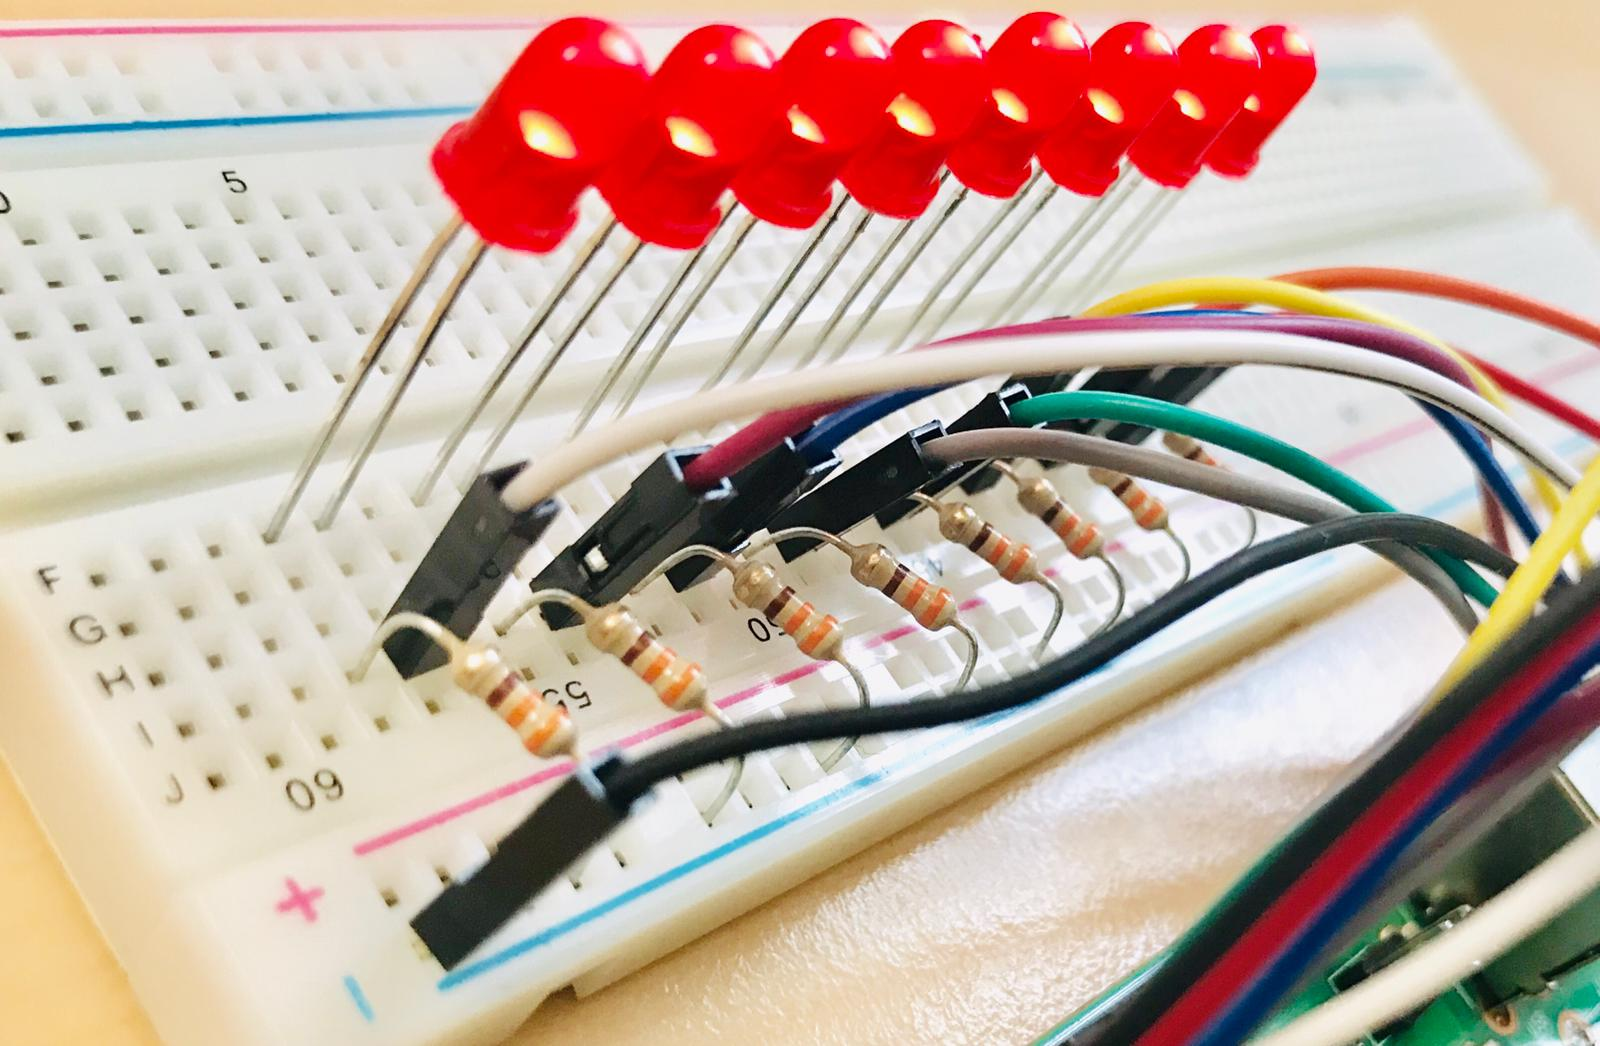
\includegraphics[width=0.6\textwidth]{/Users/allexoliveira/PharoThingsBook/Booklet-APharoThingTutorial/_result/pdf/Chapters/Chap5LEDFlowingLights/figures/pharothings-raspberry-raspberry-leds-breadboard-02.jpeg}\caption{LEDs turn On.\label{8LEDs}}\end{center}
\end{figure}

\section{Adding features}
Every time you run this code, the LEDs toggles the state, from Off to On or vice versa. Let’s reduce the delay time and add the \textcode{timesRepeat:} method, as we did in the last lesson, to repeat the alternation as many times as we want:

\begin{displaycode}{plain}
[ 2 timesRepeat: [
    gpioArray do: [ :item | item toggleDigitalValue. (Delay forSeconds: 0.1) wait ].
] ] forkNamed: 'FlowingProcess'.
\end{displaycode}

Execute this code and… cool! Now your LEDs are flowing On and Off!
\section{Reversing the flow}
We can have more fun with this experiment by changing the order of where to start changing the value of LEDs. To do this is very easy, just call the method \textcode{reverseDo:} and it will solve all for you:

\begin{displaycode}{plain}
[ 2 timesRepeat: [
    gpioArray reverseDo: [ :item | item toggleDigitalValue. (Delay forSeconds: 0.1) wait ].
] ] forkNamed: 'FlowingProcess'.
\end{displaycode}

Execute this code and… cool! Now your LEDs are flowing on reverse order!
\section{Going and backing the flow}
To finish this experiment, let’s combine the flowing On and Off with the Reverse!

\begin{displaycode}{plain}
[ 2 timesRepeat: [
    gpioArray do: [ :item | item toggleDigitalValue. (Delay forSeconds: 0.1) wait ].
    gpioArray reverseDo: [ :item | item toggleDigitalValue. (Delay forSeconds: 0.1) wait ].
] ] forkNamed: 'FlowingProcess'.
\end{displaycode}

Execute this code and… cool! Now your LEDs are flowing On and Off and on normal and reverse order!

We can improve this code. Do you see this part where the code is repeating \symbol{34}\textcode{{[} :item \textbar{} item toggleDigitalValue. (Delay forSeconds: 0.1) wait {]}}\symbol{34} ? Let's put this inside a variable named \textcode{action}, so we can call it when we want:

\begin{displaycode}{plain}
action := [ :item | item toggleDigitalValue. (Delay forSeconds: 0.1) wait ].
[ 2 timesRepeat: [
    gpioArray do: action.
    gpioArray reverseDo: action.
] ] forkNamed: 'FlowingProcess'.
\end{displaycode}

We can put the code inside the block closure \symbol{34}{[} {]} in a variable also and call it in just one line. Let's put it inside the variable \textcode{flowing}:

\begin{displaycode}{plain}
action := [ :item | item toggleDigitalValue. (Delay forSeconds: 0.1) wait ].
flowing := [ 2 timesRepeat: [
    gpioArray do: action.
    gpioArray reverseDo: action.
] ].
\end{displaycode}

Now we can start the process just send the method forkNamed: to the object \textcode{flowing}, like in the following line:

\begin{displaycode}{plain}
flowing forkNamed: 'FlowingProcess'.
\end{displaycode}

Your final code will seem like the Picture \ref{Process8LEDs}. Run this code once and when you want to flow the LEDs again, just run the last line. But remember, to each change in the code, you need to run the part that you changed. 

\begin{displaycode}{plain}
gpioArray := { gpio0. gpio1. gpio2. gpio3. gpio4. gpio5. gpio6. gpio7 }.
gpioArray do: [ :item | item beDigitalOutput ].
action := [ :item | item toggleDigitalValue. (Delay forSeconds: 0.1) wait ].
flowing := [ 2 timesRepeat: [
	gpioArray do: action.
	gpioArray reverseDo: action.
] ].
\end{displaycode}


\begin{figure}

\begin{center}
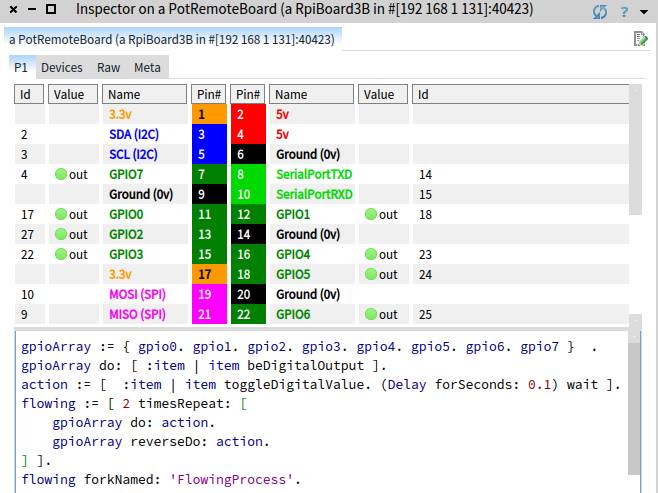
\includegraphics[width=0.85\textwidth]{/Users/allexoliveira/PharoThingsBook/Booklet-APharoThingTutorial/_result/pdf/Chapters/Chap5LEDFlowingLights/figures/pharothings-raspberry-8leds-code-lesson-02.png}\caption{Process Browser terminate.\label{Process8LEDs}}\end{center}
\end{figure}

\section{Terminating the process}
As we saw in the Blinking LED lesson, you can finish this process remotely, case you don’t want to wait it finish. To do this, call the Remote Process Browser:

\begin{displaycode}{plain}
remotePharo openProcessBrowser.
\end{displaycode}

Search the FlowingProcess and terminate it, like in Picture \ref{Inspector8LEDsfinal}, using one of these options:

\begin{itemize}
\item selecting the process and using the shortcut “Cmd + T”;
\item selecting the process and using the button Terminate;
\item or right-click and select Terminate.
\end{itemize}


\begin{figure}

\begin{center}
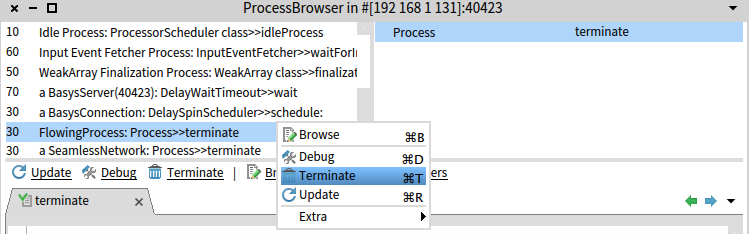
\includegraphics[width=0.8\textwidth]{/Users/allexoliveira/PharoThingsBook/Booklet-APharoThingTutorial/_result/pdf/Chapters/Chap5LEDFlowingLights/figures/pharothings-raspberry-remoteprocess.png}\caption{Process Browser terminate.\label{Inspector8LEDsfinal}}\end{center}
\end{figure}

\section{In the next lesson}
In this tutorial, you learned how to use an Array and control 8 objects at the same time by typing some code in the remote inspector. But with Pharo we can do more!

You can create your own program in classes and methods using the codes you learned in this lesson. Go ahead and try to do this yourself to test your knowledge.

And in the next lesson, let’s use object-oriented programming, OOP to create a simple program, using these codes, to control the flow like as we want.


% lulu requires an empty page at the end. That's why I'm using
% \backmatter here.
\backmatter

% Index would go here

\end{document}
